
%\begin{tikzpicture}
%\begin{axis}[
% x dir=reverse,
%  y dir=reverse,
%  grid = both,
%%  ymode=log,
%%  log basis y={50}
%  ]
%
%\addplot [
%point meta=explicit symbolic,
%scatter, only marks,
%mark=text,
%scatter/@pre marker code/.code={\pgfplotsset{text mark=\textipa{\pgfplotspointmeta}}},
%scatter/@post marker code/.code={}
%] table [x=F2, 
%y=F1, 
%col sep=comma,
%meta=phoneme] {data/julio/p1.mean.csv};
%
%
%\end{axis}
%
%\end{tikzpicture}

\begin{figure}
\def\minx{650}
\def\minxstep{700}

\subfloat[]{\noindent
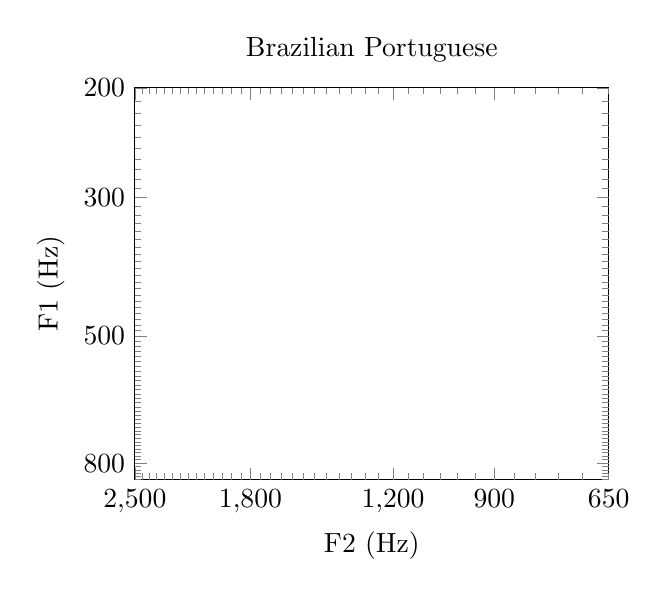
\begin{tikzpicture}
\begin{axis}[
title=Brazilian Portuguese,
xmode=log,
width=7.6cm,
ylabel=F1 (Hz),
xlabel=F2 (Hz),
ymode=log,
log basis y={2},
x dir=reverse,
y dir=reverse,
xmin=\minx,
xmax=2500,
ymin=200,
ymax=850,
extra y tick style={%
    fill=white,
    label=none,
    draw=none,
    tickwidth=0.8mm,
    fill opacity=0,
},
extra x tick style={%
    fill=white,
    label=none,
    draw=none,
    tickwidth=0.8mm,
    fill opacity=0,
},
ytick={200,300,500,800},
xtick={\minx,900,1200,1800, 2500},,
extra y ticks={200,210,...,850},
extra x ticks={\minx,\minxstep,...,2500},
yminorticks=true,
log ticks with fixed point,
]

\plotallphonemes{data/julio/p1.median.csv}

\end{axis}
\end{tikzpicture}\label{fig:bp}} \subfloat[]{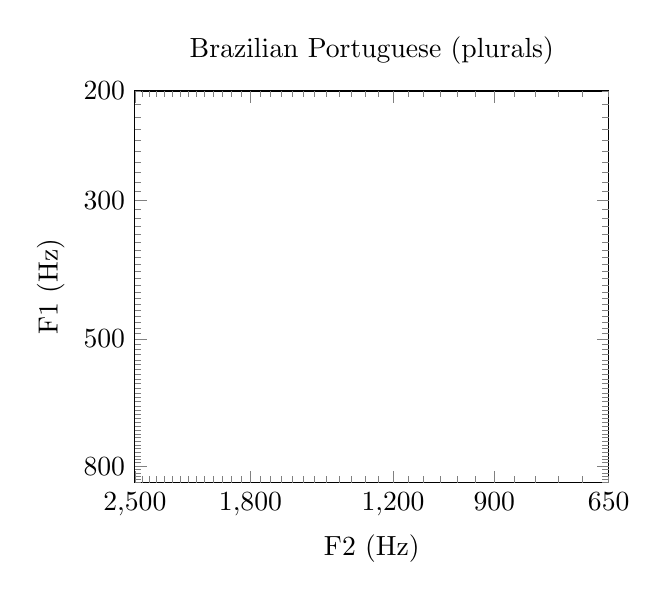
\begin{tikzpicture}
\begin{axis}[
title=Brazilian Portuguese (plurals),
xmode=log,
width=7.6cm,
ylabel=F1 (Hz),
xlabel=F2 (Hz),
ymode=log,
log basis y={2},
x dir=reverse,
y dir=reverse,
xmin=\minx,
xmax=2500,
ymin=200,
ymax=850,
extra y tick style={%
    fill=white,
    label=none,
    draw=none,
    tickwidth=0.8mm,
    fill opacity=0,
},
extra x tick style={%
    fill=white,
    label=none,
    draw=none,
    tickwidth=0.8mm,
    fill opacity=0,
},
ytick={200,300,500,800},
xtick={\minx,900,1200,1800, 2500},
extra y ticks={200,210,...,850},
extra x ticks={\minx,\minxstep,...,2500},
yminorticks=true,
log ticks with fixed point,
]

\plotallphonemes{data/julio/p2.median.csv}

\end{axis}
\end{tikzpicture}\label{fig:bps}}


\subfloat[]{\noindent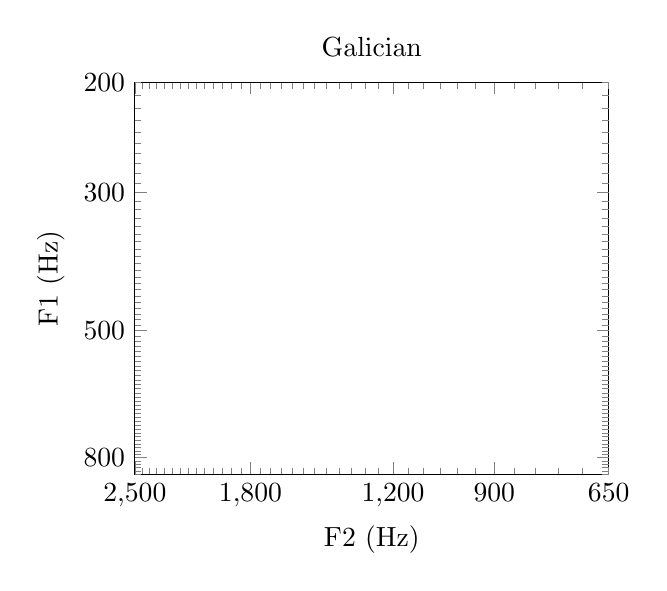
\begin{tikzpicture}
\begin{axis}[
title=Galician,
xmode=log,
width=7.6cm,
ylabel=F1 (Hz),
xlabel=F2 (Hz),
ymode=log,
log basis y={2},
x dir=reverse,
y dir=reverse,
xmin=\minx,
xmax=2500,
ymin=200,
ymax=850,
extra y tick style={%
    fill=white,
    label=none,
    draw=none,
    tickwidth=0.8mm,
    fill opacity=0,
},
extra x tick style={%
    fill=white,
    label=none,
    draw=none,
    tickwidth=0.8mm,
    fill opacity=0,
},
ytick={200,300,500,800},
xtick={\minx,900,1200,1800, 2500},,
extra y ticks={200,210,...,850},
extra x ticks={\minx,\minxstep,...,2500},
yminorticks=true,
log ticks with fixed point,
]

\plotallphonemes{data/pedro/p1.median.csv}

\end{axis}
\end{tikzpicture}\label{fig:gl}}\subfloat[]{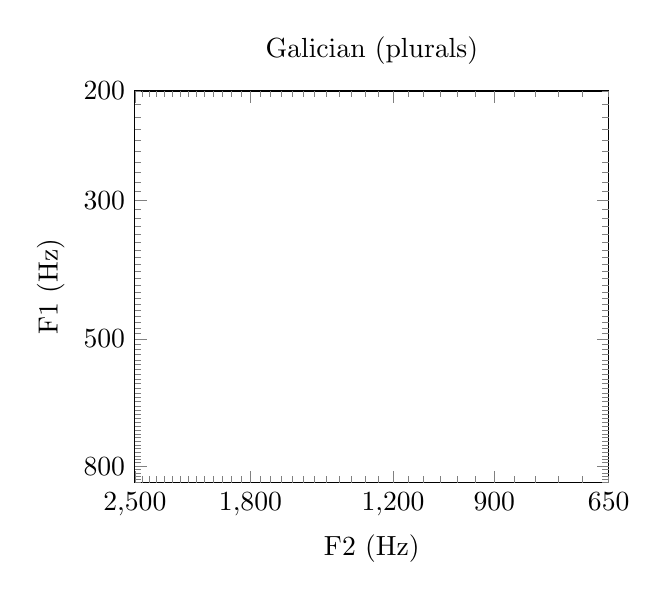
\begin{tikzpicture}
\begin{axis}[
title=Galician (plurals),
xmode=log,
width=7.6cm,
ylabel=F1 (Hz),
xlabel=F2 (Hz),
ymode=log,
log basis y={2},
x dir=reverse,
y dir=reverse,
xmin=\minx,
xmax=2500,
ymin=200,
ymax=850,
extra y tick style={%
    fill=white,
    label=none,
    draw=none,
    tickwidth=0.8mm,
    fill opacity=0,
},
extra x tick style={%
    fill=white,
    label=none,
    draw=none,
    tickwidth=0.8mm,
    fill opacity=0,
},
ytick={200,300,500,800},
xtick={\minx,900,1200,1800, 2500},,
extra y ticks={200,210,...,850},
extra x ticks={\minx,\minxstep,...,2500},
yminorticks=true,
log ticks with fixed point,]

\plotallphonemes{data/pedro/p2.median.csv}

\end{axis}
\end{tikzpicture}\label{fig:gls}}

\subfloat[]{\noindent
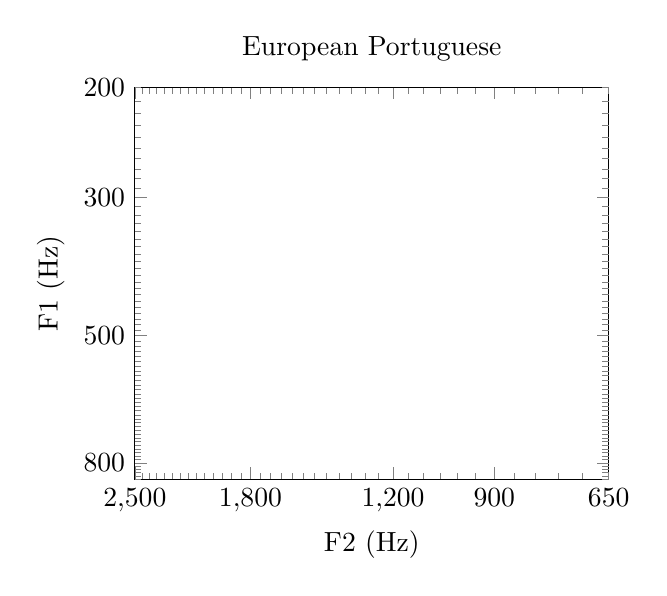
\begin{tikzpicture}
\begin{axis}[
title=European Portuguese,
xmode=log,
width=7.6cm,
ylabel=F1 (Hz),
xlabel=F2 (Hz),
ymode=log,
log basis y={2},
x dir=reverse,
y dir=reverse,
xmin=\minx,
xmax=2500,
ymin=200,
ymax=850,
extra y tick style={%
    fill=white,
    label=none,
    draw=none,
    tickwidth=0.8mm,
    fill opacity=0,
},
extra x tick style={%
    fill=white,
    label=none,
    draw=none,
    tickwidth=0.8mm,
    fill opacity=0,
},
ytick={200,300,500,800},
xtick={\minx,900,1200,1800, 2500},,
extra y ticks={200,210,...,850},
extra x ticks={\minx,\minxstep,...,2500},
yminorticks=true,
log ticks with fixed point,
]

\plotallphonemes{data/joao/p1.median.csv}

\end{axis}
\end{tikzpicture}\label{fig:ep}}\subfloat[]{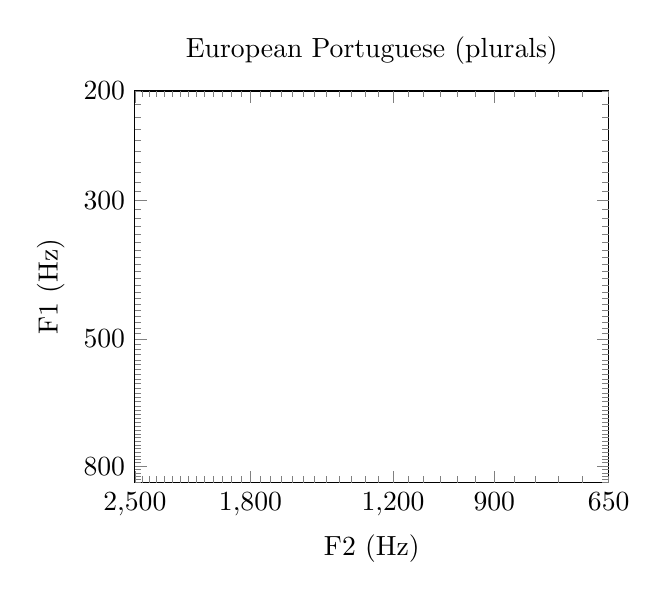
\begin{tikzpicture}
\begin{axis}[
title=European Portuguese (plurals),
xmode=log,
width=7.6cm,
ylabel=F1 (Hz),
xlabel=F2 (Hz),
ymode=log,
log basis y={2},
x dir=reverse,
y dir=reverse,
xmin=\minx,
xmax=2500,
ymin=200,
ymax=850,
extra y tick style={%
    fill=white,
    label=none,
    draw=none,
    tickwidth=0.8mm,
    fill opacity=0,
},
extra x tick style={%
    fill=white,
    label=none,
    draw=none,
    tickwidth=0.8mm,
    fill opacity=0,
},
ytick={200,300,500,800},
xtick={\minx,900,1200,1800, 2500},,
extra y ticks={200,210,...,850},
extra x ticks={\minx,\minxstep,...,2500},
yminorticks=true,
log ticks with fixed point,]

\plotallphonemes{data/joao/p2.median.csv}

\end{axis}
\end{tikzpicture}\label{fig:eps}}

\caption{First and second formants of the Brazilian, Galician and Portuguese speakers.}
\label{fig:formants}

\end{figure}
